% ================================= chapter 4 ================================= %
\chapter{シミュレーション}
目標値変更、振り上げ制御のシミュレーションを行い、重み行列、オブザーバの極、サンプリング周期、
パラメータ$k$, $n$を変更し、それぞれの変更による性能の違いを確かめる.

\subsection{重み行列変更に関するシミュレーション}
目標値変更における安定化制御で、表\ref{sim_Q}に示すパラメータを用いてシミュレーションを行う。

\begin{table}[htbp]
    \begin{center}
        \caption{表\ref{sim_Q}: 重み行列によるシミュレーションに用いるパラメータの種類}
        \begin{tabular}{|c|c|c|c|c|} \hline
            パターン & 重み行列$Q$ & オブザーバの極$P$ & サンプリング周期$dt$[s] \\ \hline \hline
            パターン1 & $Q_1$(1E6, 1E5, 1, 1) & $P_1$((-23,0), (-23,0)) & $dt_1$:0.005 \\ \hline
            パターン2 & $Q_2$(1E5, 1E6, 1, 1) & $P_2$((-23,0), (-23,0)) & $dt_2$:0.005 \\ \hline
            パターン3 & $Q_3$(1E6, 1E6, 1, 1) & $P_3$((-23,0), (-23,0)) & $dt_3$:0.005 \\ \hline
        \end{tabular}
        \label{sim_Q}
    \end{center}
\end{table}

表\ref{sim_Q}に従ってシミュレーションを行った結果を図\ref{sim_Q_r}, 図\ref{sim_Q_th}に示す。

\begin{figure}[htbp]
    \begin{minipage}{0.5\hsize}
        \begin{center}
            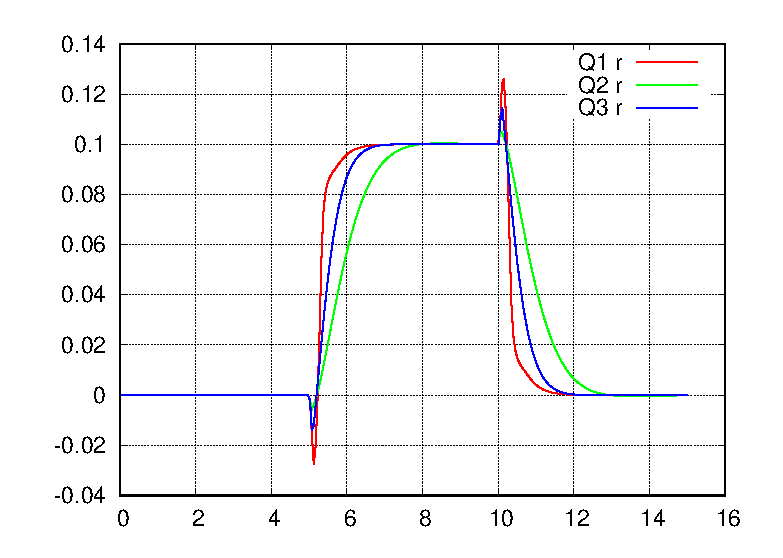
\includegraphics[width=1.0\linewidth]{CompareQ_r.eps}
            \caption{図\ref{sim_Q_r}: 重み行列による比較(台車位置)}
            \label{sim_Q_r}
        \end{center}
    \end{minipage}
    \begin{minipage}{0.5\hsize}
        \begin{center}
            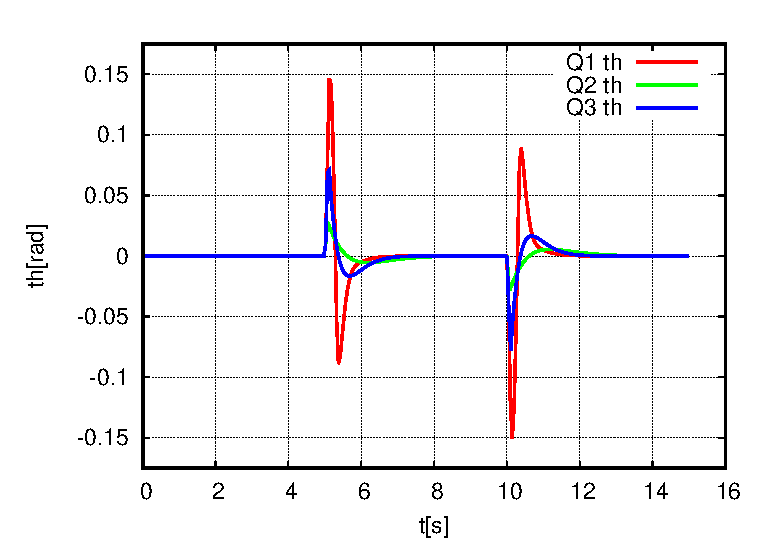
\includegraphics[width=1.0\linewidth]{CompareQ_th.eps}
            \caption{図\ref{sim_Q_th}: 重み行列による比較(振子角度})
            \label{sim_Q_th}
        \end{center}
    \end{minipage}
\end{figure}

図\ref{sim_Q_r}から、最も重みを大きくしたパターン1をみると、たしかに台車の目標位置への収束は速くなっているが、
台車の位置を有線する一方で振子の角度の振幅は大きくなっている。一方で、振子角度の重みを最も大きくしたパターン2では、
振子角度の振幅は小さく抑えられていると同時に、台車位置の目標値への収束が3パターンの中で最も遅くなっている。

\subsection{オブザーバの極変更に関するシミュレーション}
目標値変更における安定化制御で、表\ref{sim_P}に示すパラメータを用いてシミュレーションを行う。

\begin{table}[htbp]
    \begin{center}
        \caption{表\ref{sim_P}: オブザーバの極によるシミュレーションに用いるパラメータの種類}
        \begin{tabular}{|c|c|c|c|c|} \hline
            パターン & 重み行列$Q$ & オブザーバの極$P$ & サンプリング周期$dt$[s] \\ \hline \hline
            パターン1 & $Q_1$(1E6, 1E5, 1, 1) & $P_1$((-23,0), (-23,0)) & $dt_1$:0.005 \\ \hline
            パターン2 & $Q_2$(1E6, 1E5, 1, 1) & $P_2$((-50,0), (-50,0)) & $dt_2$:0.005 \\ \hline
        \end{tabular}
        \label{sim_P}
    \end{center}
\end{table}

表\ref{sim_P}に従ってシミュレーションを行った結果を図\ref{sim_P_r}, 図\ref{sim_P_th}に示す。

\begin{figure}[htbp]
    \begin{minipage}{0.5\hsize}
        \begin{center}
            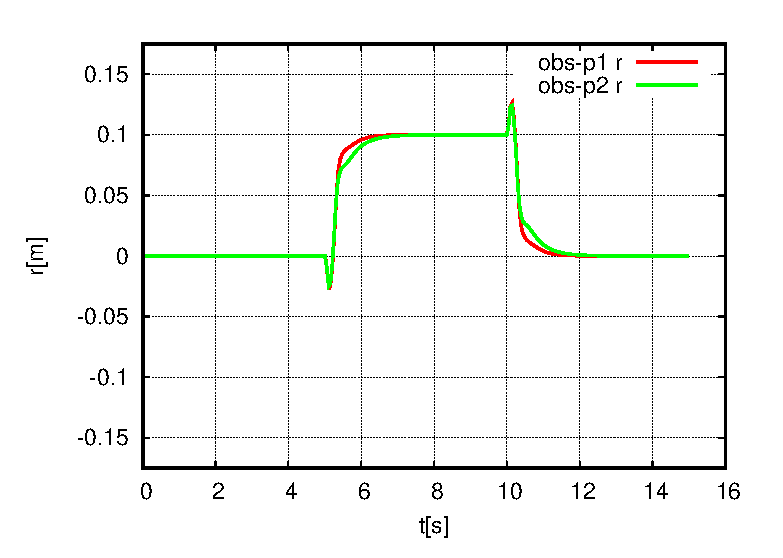
\includegraphics[width=1.0\linewidth]{CompareP_r.eps}
            \caption{図\ref{sim_P_r}: オブザーバの極による比較(台車位置)}
            \label{sim_P_r}
        \end{center}
    \end{minipage}
    \begin{minipage}{0.5\hsize}
        \begin{center}
            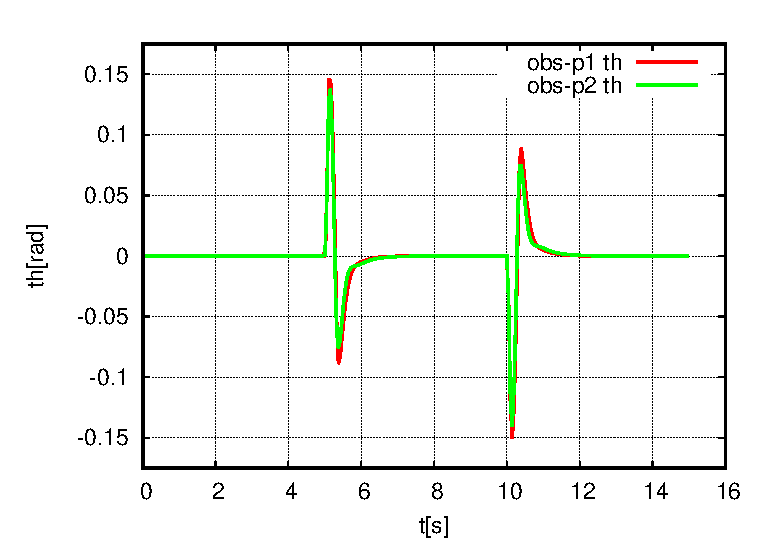
\includegraphics[width=1.0\linewidth]{CompareP_th.eps}
            \caption{図\ref{sim_P_th}: オブザーバの極による比較(振子角度)}
            \label{sim_P_th}
        \end{center}
    \end{minipage}
\end{figure}

台車位置、振子角度だけでは変化が表れにくいので、それぞれのオブザーバの推定誤差を用いて比較を行う。
図\ref{error_obs_r}に台車速度に関する推定誤差を、図\ref{error_obs_th}に振子角速度に関する推定誤差を示す。

\begin{figure}[htbp]
    \begin{minipage}{0.5\hsize}
        \begin{center}
            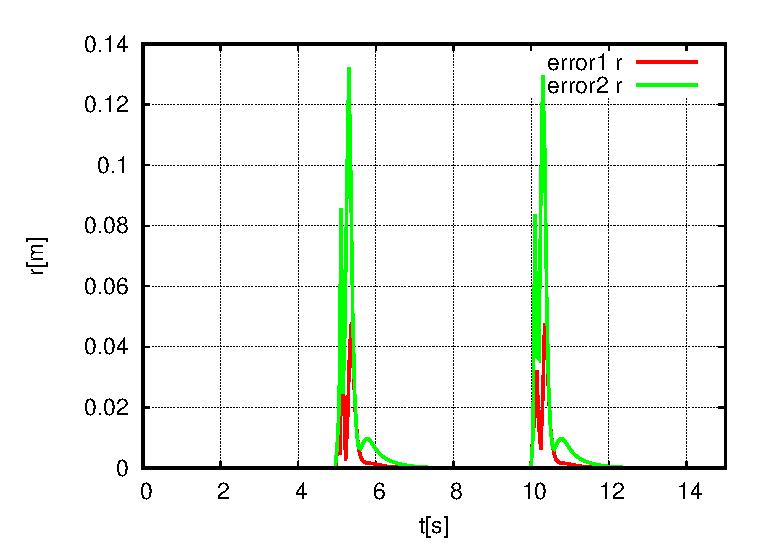
\includegraphics[width=1.0\linewidth]{error_obs_r.eps}
            \caption{図\ref{error_obs_r}: 台車速度の推定誤差}
            \label{error_obs_r}
        \end{center}
    \end{minipage}
    \begin{minipage}{0.5\hsize}
        \begin{center}
            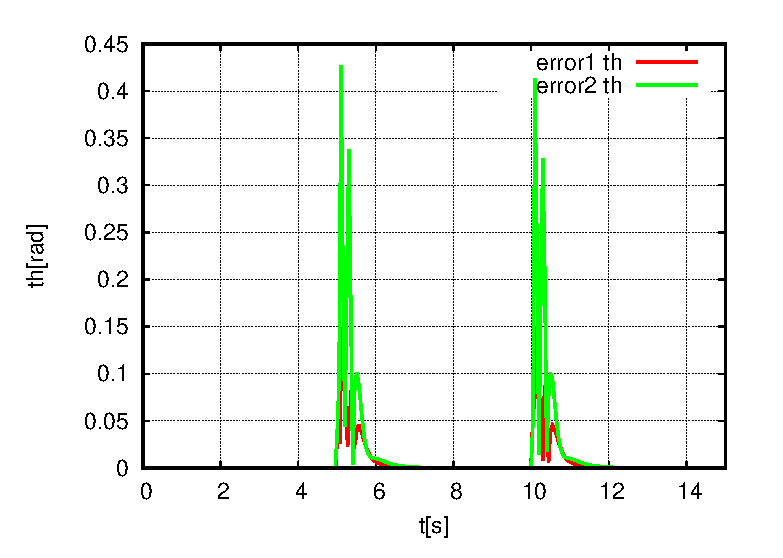
\includegraphics[width=1.0\linewidth]{error_obs_th.eps}
            \caption{図\ref{error_obs_th}: 振子角速度の推定誤差}
            \label{error_obs_th}
        \end{center}
    \end{minipage}
\end{figure}

台車速度、振子角度の推定誤差ともに、オブザーバの極が負の方向に虚軸から遠いほど推定誤差が大きくなっている。
よって、このシミュレーション結果からはオブザーバの極は虚軸に近い極配置が好ましいと言える。
実際には、極の絶対値がより大きいほど推定誤差は小さくなるが、本実験で行ったシミュレーションのパラメータでは
既に極の絶対値が十分に大きく、オブザーバの極配置以外の要因により推定誤差が大きくなったと考察できる。


\subsection{サンプリング周期変更に関するシミュレーション}
目標値変更における安定化制御で、表\ref{sim_Dt}に示すパラメータを用いてシミュレーションを行う。

\begin{table}[htbp]
    \begin{center}
        \caption{表\ref{sim_Dt}: サンプリング周期によるシミュレーションに用いるパラメータの種類}
        \begin{tabular}{|c|c|c|c|c|} \hline
            パターン & 重み行列$Q$ & オブザーバの極$P$ & サンプリング周期$dt$[s] \\ \hline \hline
            パターン1 & $Q_1$(1E6, 1E5, 1, 1) & $P_1$((-23,0), (-23,0)) & $dt_1$:0.005 \\ \hline
            パターン2 & $Q_2$(1E6, 1E5, 1, 1) & $P_2$((-23,0), (-23,0)) & $dt_2$:0.01 \\ \hline
        \end{tabular}
        \label{sim_Dt}
    \end{center}
\end{table}

表\ref{sim_Dt}に従ってシミュレーションを行った結果を図\ref{sim_Dt_r}, 図\ref{sim_Dt_th}に示す。

\begin{figure}[htbp]
    \begin{minipage}{0.5\hsize}
        \begin{center}
            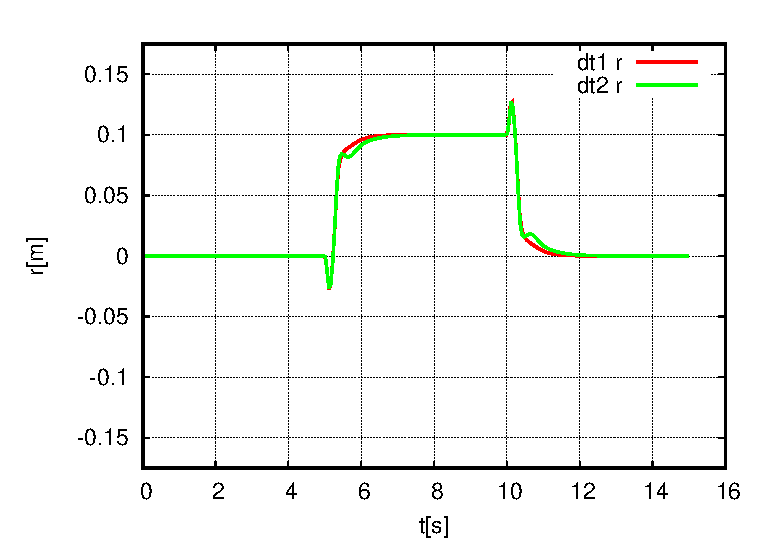
\includegraphics[width=1.0\linewidth]{CompareDt_r.eps}
            \caption{図\ref{sim_Dt_r}: サンプリング周期による比較(台車位置)}
            \label{sim_Dt_r}
        \end{center}
    \end{minipage}
    \begin{minipage}{0.5\hsize}
        \begin{center}
            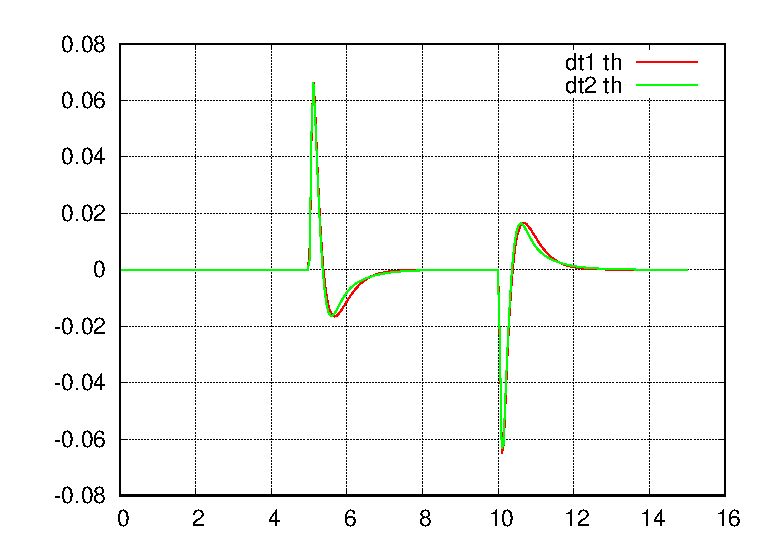
\includegraphics[width=1.0\linewidth]{CompareDt_th.eps}
            \caption{図\ref{sim_Dt_th}: サンプリング周期による比較(振子角度)}
            \label{sim_Dt_th}
        \end{center}
    \end{minipage}
\end{figure}

オブザーバの極によるシミュレーション同様、台車位置、振子角度だけでは変化が表れにくいので、
それぞれのオブザーバの推定誤差を用いて比較を行う。
図\ref{error_dt_r}に台車速度に関する推定誤差を、図\ref{error_dt_th}に振子角速度に関する推定誤差を示す。

\begin{figure}[htbp]
    \begin{minipage}{0.5\hsize}
        \begin{center}
            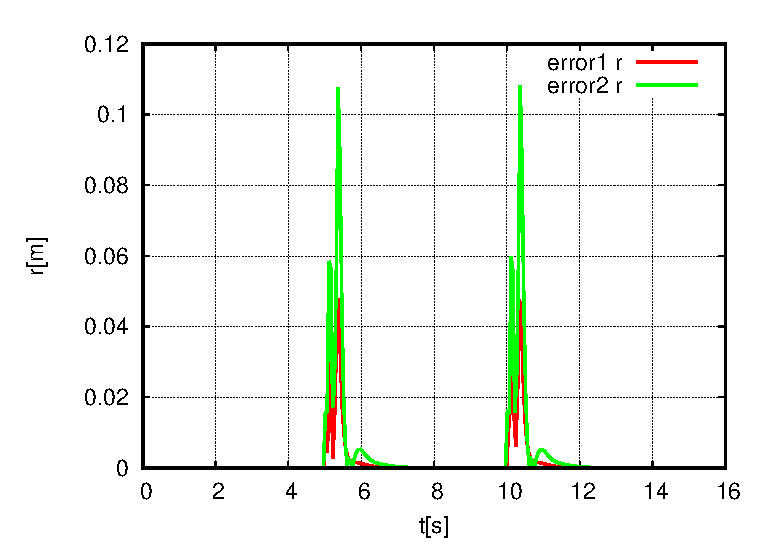
\includegraphics[width=1.0\linewidth]{error_dt_r.eps}
            \caption{図\ref{error_dt_r}: 台車速度の推定誤差}
            \label{error_dt_r}
        \end{center}
    \end{minipage}
    \begin{minipage}{0.5\hsize}
        \begin{center}
            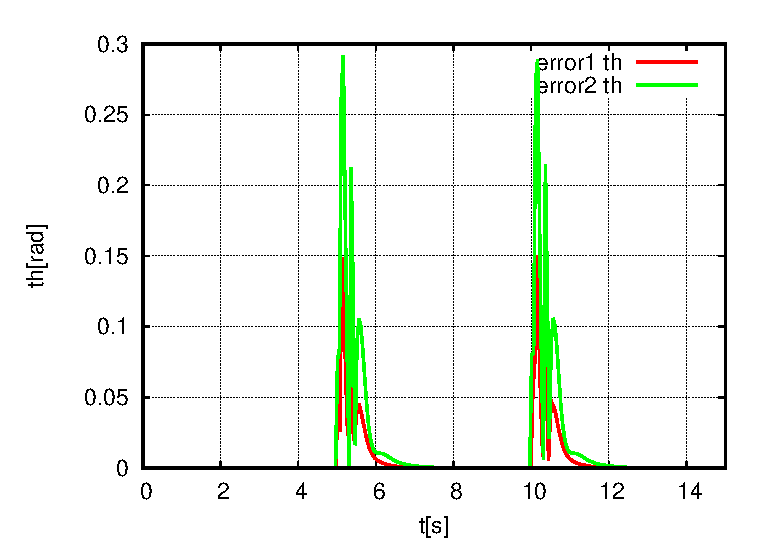
\includegraphics[width=1.0\linewidth]{error_dt_th.eps}
            \caption{図\ref{error_dt_th}: 振子角速度の推定誤差}
            \label{error_dt_th}
        \end{center}
    \end{minipage}
\end{figure}

図\ref{error_dt_r},図\ref{error_dt_th}から、サンプリング周期が短いほど推定誤差が小さくなっている。
サンプリング周期を大きくすると、計測するデータの間隔が大きくなってしまうため、実際の値への追従が遅れる。
よって、このシミュレーションでは意図した結果が得られたと言える。


\subsection{振り上げ制御のシミュレーション}
振り上げシミュレーションに用いたパラメータを表\ref{sim_swing}に示す。
ただし、振子が安定化制御に移行した際に用いるパラメータは表\ref{swing_stable}のパラメータを用いることとする。
また、台車位置、振子角度の制限として、台車位置はベルト中心から両方向に$0.09$[m],振子角度は
$\left[-\pi\right.,\ \left.\pi\right)$[rad]の範囲の値を取るものとする。

\begin{table}[htbp]
    \begin{center}
        \caption{表\ref{sim_swing}: 振り上げ制御のシミュレーションに用いるパラメータの種類}
        \begin{tabular}{|c|c|c|} \hline
            パターン & $k$ & $n$ \\ \hline \hline
            パターン1 & $1.0\mbox{E}3$ & $0.31$ \\ \hline
            パターン2 & $1.0\mbox{E}4$ & $0.31$ \\ \hline
            パターン3 & $1.0\mbox{E}5$ & $0.31$ \\ \hline
        \end{tabular}
        \label{sim_swing}
    \end{center}
\end{table}

\begin{table}[htbp]
    \begin{center}
        \caption{表\ref{swing_stable}: 振り上げ後の安定化制御に用いるパラメータ}
        \begin{tabular}{|c|c|c|c|} \hline
            重み行列$Q$ & オブザーバの極$P$ & サンプリング周期$dt$[s] \\ \hline \hline
            $Q$(1E6, 1E5, 1, 1) & $P$((-23,0), (-23,0)) & $dt$:0.005 \\ \hline
          \end{tabular}
        \label{swing_stable}
    \end{center}
\end{table}

表\ref{sim_swing}を用いて振り上げ制御のシミュレーションを行った結果を図\ref{sim_swing_r},
図\ref{sim_swing_th}に示す。

\begin{figure}[htbp]
    \begin{minipage}{0.5\hsize}
        \begin{center}
            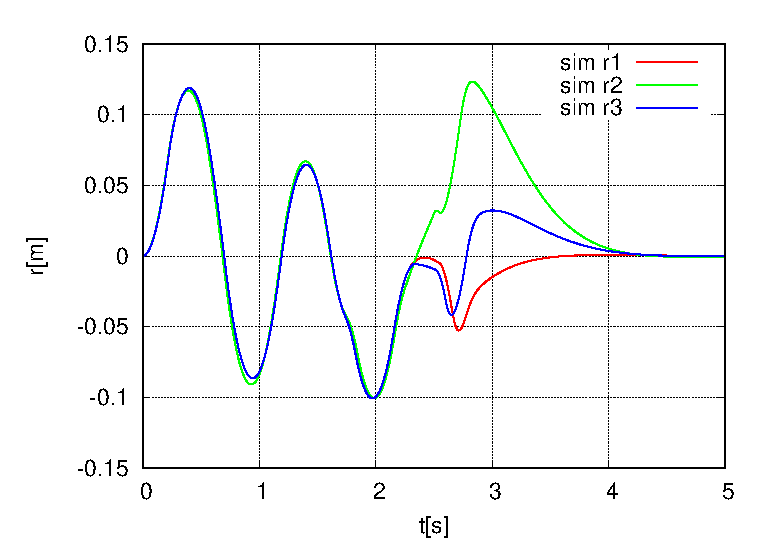
\includegraphics[width=1.0\linewidth]{swing_sim_r.eps}
            \caption{図\ref{sim_swing_r}: 台車位置}
            \label{sim_swing_r}
        \end{center}
    \end{minipage}
    \begin{minipage}{0.5\hsize}
        \begin{center}
            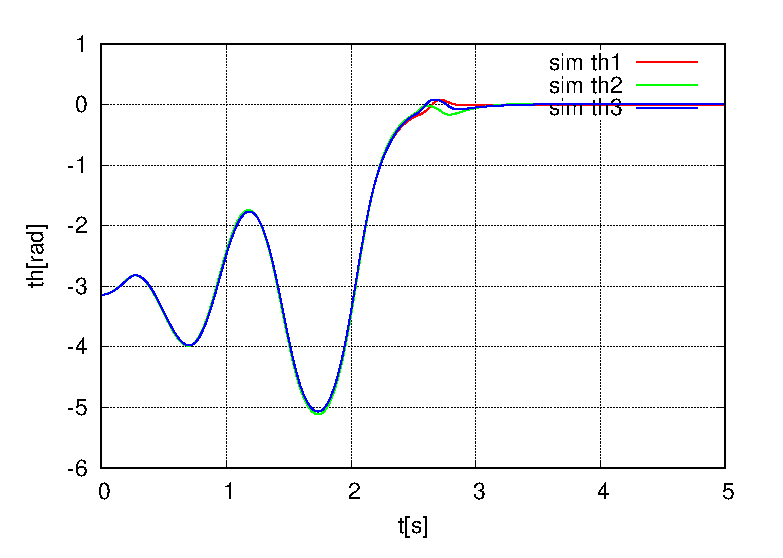
\includegraphics[width=1.0\linewidth]{swing_sim_th.eps}
            \caption{図\ref{sim_swing_th}: 振子角度}
            \label{sim_swing_th}
        \end{center}
    \end{minipage}
\end{figure}

パラメータ$k$の値を大きくすることで、目標とする振子の運動エネルギーへの収束が速くなることが予想されたが、
本実験のシミュレーションでは$k$の値に関わらず安定化制御に移行するまでの時間に変化はなかった。
ただし、安定化制御に移行する際の台車位置はそれぞれ異なっていたため、パラメータ$k$の値によっては
台車が制限された移動範囲外にはみ出してしまう可能性がある。

% =============================== chapter 4 END =============================== %